\newcommand{\gratingillumination}{
    \begin{tikzpicture}[domain=0:3.14*6/5, samples=200, scale=1]
    
        % x-axis
        \draw[->, gray, line width=1pt] (0,0) -- (4,0) node[right, gray] {$x$};
        \draw[->, gray, line width=1pt] (0,0) -- (0,1.5) node[above, gray] {$I(x)$};

        % illumination plot
        \draw[color=darkgray, densely dotted, line width=1pt]    plot (\x, {\a*sin(deg(\x/\p))+\b});

        % grating
        \draw[draw=black, line width=0.25, fill=black] (3.14 * \p, 0.7 + 0.75) rectangle (2*3.14 * \p,0.8 + 0.75);
        \draw[draw=black, line width=0.25, fill=black] (3*3.14 * \p, 0.7 + 0.75) rectangle (4*3.14 * \p,0.8 + 0.75);
        \draw[draw=black, line width=0.25, fill=black] (5*3.14 * \p, 0.7 + 0.75) rectangle (6*3.14 * \p,0.8 + 0.75);

        % descriptors
        \draw[] (3.5*3.14,1.45) node[above, black] {illumination grating};
    \end{tikzpicture}
}


\newcommand{\prismeffect}{
    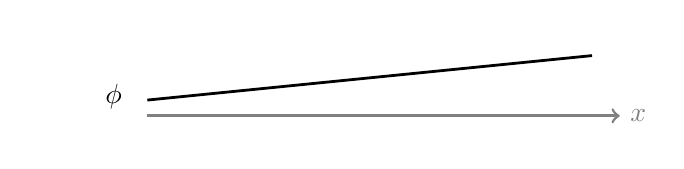
\begin{tikzpicture}[domain=0:5.65, samples=200, scale=1]
    
        % x-axis
        \draw[->, gray, line width=1pt] (0,0) -- (6,0) node[right, gray] {$x$};
        % \draw[->, gray, line width=1pt] (0,0) -- (0,1) node[right, gray] {$\phi$};

        % phase plot
        \draw[color=black, line width=1pt]    plot (\x, {0.1*\x+0.2});

        % yeah, this is smehow necessary
        \draw[color=white, fill=white] (0,1.1) circle (0.0125);
        \draw[color=white, fill=white] (0,-0.3) circle (0.0125);
        \draw[color=white, fill=white] (-1.5,0) circle (0.0125);
        % phase descriptor
        \draw (-0.2, 0.25) node[left] {$\phi$};

    \end{tikzpicture}

    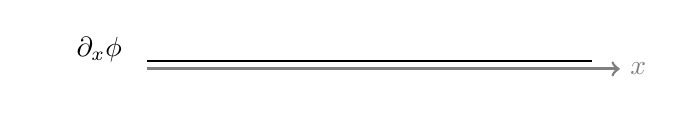
\begin{tikzpicture}[domain=0:5.65, samples=200, scale=1]
    
        % x-axis
        \draw[->, gray, line width=1pt] (0,0) -- (6,0) node[right, gray] {$x$};
        % \draw[->, gray, line width=1pt] (0,0) -- (0,1) node[right, gray] {$\phi$};

        % phase plot
        \draw[color=black, line width=1pt]    plot (\x, {0.1});

        % yeah, this is smehow necessary
        \draw[color=white, fill=white] (0,0.5) circle (0.0125);
        \draw[color=white, fill=white] (0,-0.3) circle (0.0125);
        \draw[color=white, fill=white] (-1.5,0) circle (0.0125);
        % phase descriptor
        \draw (-0.2, 0.25) node[left] {$\partial_x\phi$};

    \end{tikzpicture}

    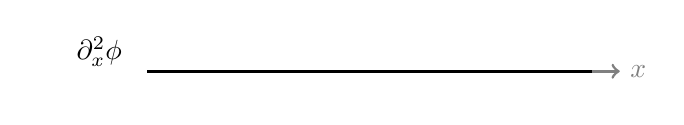
\begin{tikzpicture}[domain=0:5.65, samples=200, scale=1]
    
        % x-axis
        \draw[->, gray, line width=1pt] (0,0) -- (6,0) node[right, gray] {$x$};
        % \draw[->, gray, line width=1pt] (0,0) -- (0,1) node[right, gray] {$\phi$};

        % phase plot
        \draw[color=black, line width=1pt]    plot (\x, {0});

        % yeah, this is smehow necessary
        \draw[color=white, fill=white] (0,0.5) circle (0.0125);
        \draw[color=white, fill=white] (0,-0.3) circle (0.0125);
        \draw[color=white, fill=white] (-1.5,0) circle (0.0125);
        % phase descriptor
        \draw (-0.2, 0.25) node[left] {$\partial_x^2\phi$};

    \end{tikzpicture}
}


\newcommand{\focusingeffect}{
    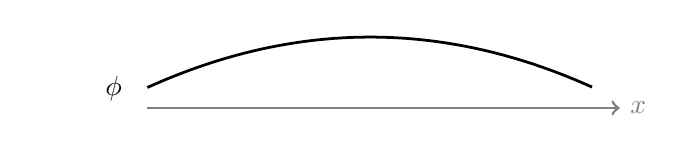
\begin{tikzpicture}[domain=0:5.65, samples=200, scale=1]
    
        % x-axis
        \draw[->, gray, line width=1pt] (0,0) -- (6,0) node[right, gray] {$x$};

        % phase plot
        \draw[color=black, line width=1pt]    plot (\x, {-0.08*(\x-2.83)^2+0.9});

        % yeah, this is smehow necessary
        \draw[color=white, fill=white] (0,1) circle (0.0125);
        \draw[color=white, fill=white] (0,-0.3) circle (0.0125);
        \draw[color=white, fill=white] (-1.5,0) circle (0.0125);
        % phase descriptor
        \draw (-0.2, 0.25) node[left] {$\phi$};

    \end{tikzpicture}

    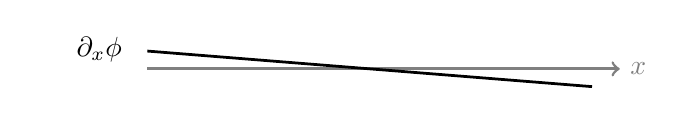
\begin{tikzpicture}[domain=0:5.65, samples=200, scale=1]
    
        % x-axis
        \draw[->, gray, line width=1pt] (0,0) -- (6,0) node[right, gray] {$x$};

        % phase plot
        \draw[color=black, line width=1pt]    plot (\x, {-0.08*(\x-2.83)});

        % yeah, this is smehow necessary
        \draw[color=white, fill=white] (0,0.5) circle (0.0125);
        \draw[color=white, fill=white] (0,-0.3) circle (0.0125);
        \draw[color=white, fill=white] (-1.5,0) circle (0.0125);
        % phase descriptor
        \draw (-0.2, 0.25) node[left] {$\partial_x\phi$};

    \end{tikzpicture}

    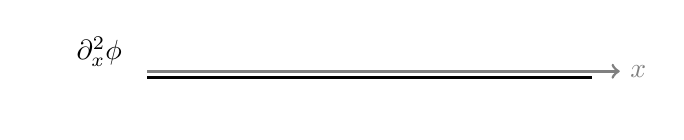
\begin{tikzpicture}[domain=0:5.65, samples=200, scale=1]
    
        % x-axis
        \draw[->, gray, line width=1pt] (0,0) -- (6,0) node[right, gray] {$x$};

        % phase plot
        \draw[color=black, line width=1pt]    plot (\x, {-0.08});

        % yeah, this is smehow necessary
        \draw[color=white, fill=white] (0,0.5) circle (0.0125);
        \draw[color=white, fill=white] (0,-0.5) circle (0.0125);
        \draw[color=white, fill=white] (-1.5,0) circle (0.0125);
        % phase descriptor
        \draw (-0.2, 0.25) node[left] {$\partial_x^2\phi$};

    \end{tikzpicture}
}


\newcommand{\edgeeffect}{
    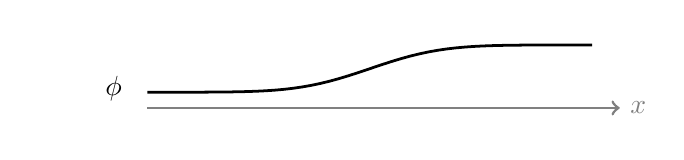
\begin{tikzpicture}[domain=0:5.65, samples=200, scale=1]
    
        % x-axis
        \draw[->, gray, line width=1pt] (0,0) -- (6,0) node[right, gray] {$x$};

        % yeah, this is smehow necessary
        \draw[color=white, fill=white] (0,1) circle (0.0125);
        \draw[color=white, fill=white] (0,-0.28) circle (0.0125);
        \draw[color=white, fill=white] (-1.5,0) circle (0.0125);
        % phase descriptor
        \draw (-0.2, 0.25) node[left] {$\phi$};

        % phase plot
        \draw[color=black, line width=1] plot coordinates {
(0.0, 0.2000188249238164)
(0.1153061224489796, 0.20003703725621974)
(0.2306122448979592, 0.2000710509618709)
(0.3459183673469388, 0.2001329122699222)
(0.4612244897959184, 0.20024247454886773)
(0.576530612244898, 0.20043143889190362)
(0.6918367346938776, 0.2007488159639757)
(0.8071428571428572, 0.201267912527476)
(0.9224489795918368, 0.20209470727368029)
(1.0377551020408164, 0.20337710944259618)
(1.153061224489796, 0.20531410127722888)
(1.2683673469387755, 0.20816320574815383)
(1.3836734693877553, 0.2122442003718416)
(1.4989795918367348, 0.21793667048765036)
(1.6142857142857143, 0.2256690401248458)
(1.729591836734694, 0.23589729603979304)
(1.8448979591836736, 0.24907281453402486)
(1.9602040816326531, 0.265600460891603)
(2.075510204081633, 0.2857902364558488)
(2.190816326530612, 0.30980781209875063)
(2.306122448979592, 0.3376308182216625)
(2.4214285714285717, 0.36901827687617916)
(2.536734693877551, 0.4034997238600805)
(2.6520408163265308, 0.4403883128699934)
(2.7673469387755105, 0.47881879584934)
(2.88265306122449, 0.5178073276745775)
(2.9979591836734696, 0.5563263416598552)
(3.1132653061224493, 0.5933850844400891)
(3.2285714285714286, 0.6281053820972656)
(3.3438775510204084, 0.659783066732673)
(3.459183673469388, 0.6879280275951896)
(3.5744897959183675, 0.7122794921708099)
(3.689795918367347, 0.7327971003753213)
(3.805102040816327, 0.7496318079219788)
(3.9204081632653063, 0.7630830256990626)
(4.035714285714286, 0.7735493647837266)
(4.151020408163266, 0.781479948416061)
(4.266326530612245, 0.787331790947885)
(4.381632653061224, 0.7915367059892933)
(4.496938775510205, 0.7944790870073846)
(4.612244897959184, 0.7964841021696047)
(4.727551020408163, 0.7978145978002249)
(4.842857142857143, 0.7986743756595149)
(4.958163265306123, 0.799215423970107)
(5.073469387755102, 0.7995469844703709)
(5.188775510204082, 0.7997448483167182)
(5.3040816326530615, 0.7998598348535066)
(5.419387755102041, 0.7999249083870964)
(5.534693877551021, 0.79996077072501)
(5.65, 0.799980017128178)
        };
    \end{tikzpicture}

    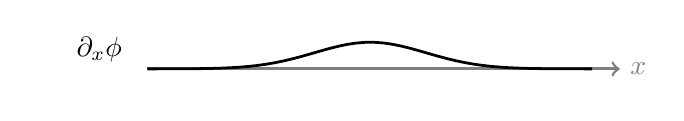
\begin{tikzpicture}[domain=0:5.65, samples=200, scale=1]
    
        % x-axis
        \draw[->, gray, line width=1pt] (0,0) -- (6,0) node[right, gray] {$x$};

        % yeah, this is smehow necessary
        \draw[color=white, fill=white] (0,0.5) circle (0.0125);
        \draw[color=white, fill=white] (0,-0.28) circle (0.0125);
        \draw[color=white, fill=white] (-1.5,0) circle (0.0125);
        % phase descriptor
        \draw (-0.2, 0.25) node[left] {$\partial_x\phi$};

        % phase plot
        \draw[color=black, line width=1] plot coordinates {
(0.0, 0.00011260887301633994)
(0.1153061224489796, 0.00021340996889995803)
(0.2306122448979592, 0.00039383039964702165)
(0.3459183673469388, 0.0007077114352832538)
(0.4612244897959184, 0.001238384858189834)
(0.576530612244898, 0.002110121666188958)
(0.6918367346938776, 0.003501158754458667)
(0.8071428571428572, 0.005656770427830416)
(0.9224489795918368, 0.008899748777560503)
(1.0377551020408164, 0.01363450528684529)
(1.153061224489796, 0.020340117867699296)
(1.2683673469387755, 0.02954744883971905)
(1.3836734693877553, 0.04179640771494964)
(1.4989795918367348, 0.05757187425163069)
(1.6142857142857143, 0.07722078689558266)
(1.729591836734694, 0.100858039306595)
(1.8448979591836736, 0.12827418472011579)
(1.9602040816326531, 0.15886215464307188)
(2.075510204081633, 0.19158172429027734)
(2.190816326530612, 0.2249780511832228)
(2.306122448979592, 0.2572637921037791)
(2.4214285714285717, 0.2864637197622203)
(2.536734693877551, 0.31060828144854585)
(2.6520408163265308, 0.3279509385450377)
(2.7673469387755105, 0.3371763998205172)
(2.88265306122449, 0.33756538313740214)
(2.9979591836734696, 0.3290872695748221)
(3.1132653061224493, 0.31240408525597424)
(3.2285714285714286, 0.2887850922451255)
(3.3438775510204084, 0.2599472812685228)
(3.459183673469388, 0.22784958015535653)
(3.5744897959183675, 0.1944749324838341)
(3.689795918367347, 0.16163353443544806)
(3.805102040816327, 0.1308132554396985)
(3.9204081632653063, 0.1030918851628221)
(4.035714285714286, 0.07911332772087389)
(4.151020408163266, 0.05911902558219884)
(4.266326530612245, 0.04301870430725497)
(4.381632653061224, 0.03048174513255231)
(4.496938775510205, 0.021031719109678163)
(4.612244897959184, 0.01413065072384312)
(4.727551020408163, 0.009244895238528785)
(4.842857142857143, 0.005889714864079077)
(4.958163265306123, 0.0036537513536100135)
(5.073469387755102, 0.0022071718669564038)
(5.188775510204082, 0.0012983319899068093)
(5.3040816326530615, 0.0007436829199808371)
(5.419387755102041, 0.0004148033927242612)
(5.534693877551021, 0.00022529379766267346)
(5.65, 0.00011915399689421681)
        };
    \end{tikzpicture}

    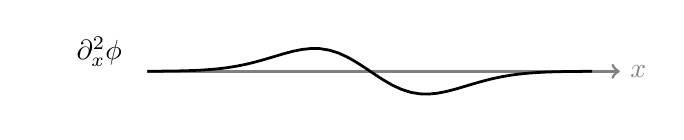
\begin{tikzpicture}[domain=0:5.65, samples=200, scale=1]
    
        % x-axis
        \draw[->, gray, line width=1pt] (0,0) -- (6,0) node[right, gray] {$x$};

        % yeah, this is smehow necessary
        \draw[color=white, fill=white] (0,0.5) circle (0.0125);
        \draw[color=white, fill=white] (0,-0.5) circle (0.0125);
        \draw[color=white, fill=white] (-1.5,0) circle (0.0125);
        % phase descriptor
        \draw (-0.2, 0.25) node[left] {$\partial_x^2\phi$};

        % phase plot
        \draw[color=black, line width=1] plot coordinates {
(0.0, 0.0006376002746610877)
(0.1153061224489796, 0.0011590615763001912)
(0.2306122448979592, 0.0020480167878256243)
(0.3459183673469388, 0.0035168862184964404)
(0.4612244897959184, 0.0058681280485639595)
(0.576530612244898, 0.009511823360036644)
(0.6918367346938776, 0.014974165429115784)
(0.8071428571428572, 0.022888105054158506)
(0.9224489795918368, 0.03395602638991969)
(1.0377551020408164, 0.048875064156100885)
(1.153061224489796, 0.06821968279946412)
(1.2683673469387755, 0.09228414317519197)
(1.3836734693877553, 0.1208992155802835)
(1.4989795918367348, 0.1532512358215499)
(1.6142857142857143, 0.18774403384869134)
(1.729591836734694, 0.2219509434369105)
(1.8448979591836736, 0.2527005523276505)
(1.9602040816326531, 0.2763231884715112)
(2.075510204081633, 0.2890557040803599)
(2.190816326530612, 0.2875644975192105)
(2.306122448979592, 0.26950946175316465)
(2.4214285714285717, 0.2340453778355567)
(2.536734693877551, 0.18215194988305264)
(2.6520408163265308, 0.1167045573751291)
(2.7673469387755105, 0.04224323743484915)
(2.88265306122449, -0.03554178423735622)
(2.9979591836734696, -0.11052824396999729)
(3.1132653061224493, -0.1769579299941149)
(3.2285714285714286, -0.23016704833138393)
(3.3438775510204084, -0.2671223249760824)
(3.459183673469388, -0.2866782559497461)
(3.5744897959183675, -0.2895316469482268)
(3.689795918367347, -0.2779110824289999)
(3.805102040816327, -0.2550861980926689)
(3.9204081632653063, -0.2248048165615635)
(4.035714285714286, -0.19076283149296883)
(4.151020408163266, -0.15618701659794734)
(4.266326530612245, -0.12357421120495761)
(4.381632653061224, -0.09459235770353792)
(4.496938775510205, -0.07011847748744639)
(4.612244897959184, -0.050370830365908954)
(4.727551020408163, -0.03508789435760496)
(4.842857142857143, -0.023712761097194338)
(4.958163265306123, -0.015553661966705159)
(5.073469387755102, -0.0099051171235931)
(5.188775510204082, -0.0061261982088056674)
(5.3040816326530615, -0.00368075269205348)
(5.419387755102041, -0.002148775755744792)
(5.534693877551021, -0.0012190926925448322)
(5.65, -0.0006722727931840479)
        };
    \end{tikzpicture}
}





